\documentclass[12pt]{report}

\usepackage[a4paper, margin=1in]{geometry}
\usepackage{graphicx}
\usepackage{amsmath}
\usepackage[hidelinks]{hyperref}
\usepackage{booktabs}
\usepackage{setspace}
\usepackage{subcaption}
\usepackage{float}
\usepackage{xparse}
\usepackage{xcolor}
\usepackage{array}

\title{Ph.D. Progress Report}
\author{Raj Singh}
\date{\today}

\begin{document}

\maketitle
\tableofcontents

\chapter{Introduction}

\begin{spacing}{1.06}
Machine learning has become a central methodology for addressing complex problems in healthcare, especially in settings where large volumes of heterogeneous data must be analyzed in a consistent and reproducible manner. Within this broader field, computer vision methods are particularly relevant because they enable automatic extraction of discriminative visual patterns from structured image-like inputs. In medicine, such approaches have already demonstrated value for diagnosis support, screening, and disease monitoring across multiple modalities~\cite{litjens2017survey, esteva2017dermatologist, lecun2015deep, shen2017deep}.

Pain drawings constitute a clinically meaningful yet comparatively underexplored visual modality. Instead of relying on radiological imaging, pain drawings encode the self-reported spatial distribution of symptoms on a standardized human body template. This makes them especially useful for disorders in which the location, spread, and symmetry of pain carry diagnostic relevance. Examples include Ehlers-Danlos syndrome, neuromuscular disorders, and rheumatological diseases, where symptom patterns are often heterogeneous and partially overlapping~\cite{wester2020pain, emmert2018pain2d}.
\end{spacing}

\begin{figure}[t]
    \centering
    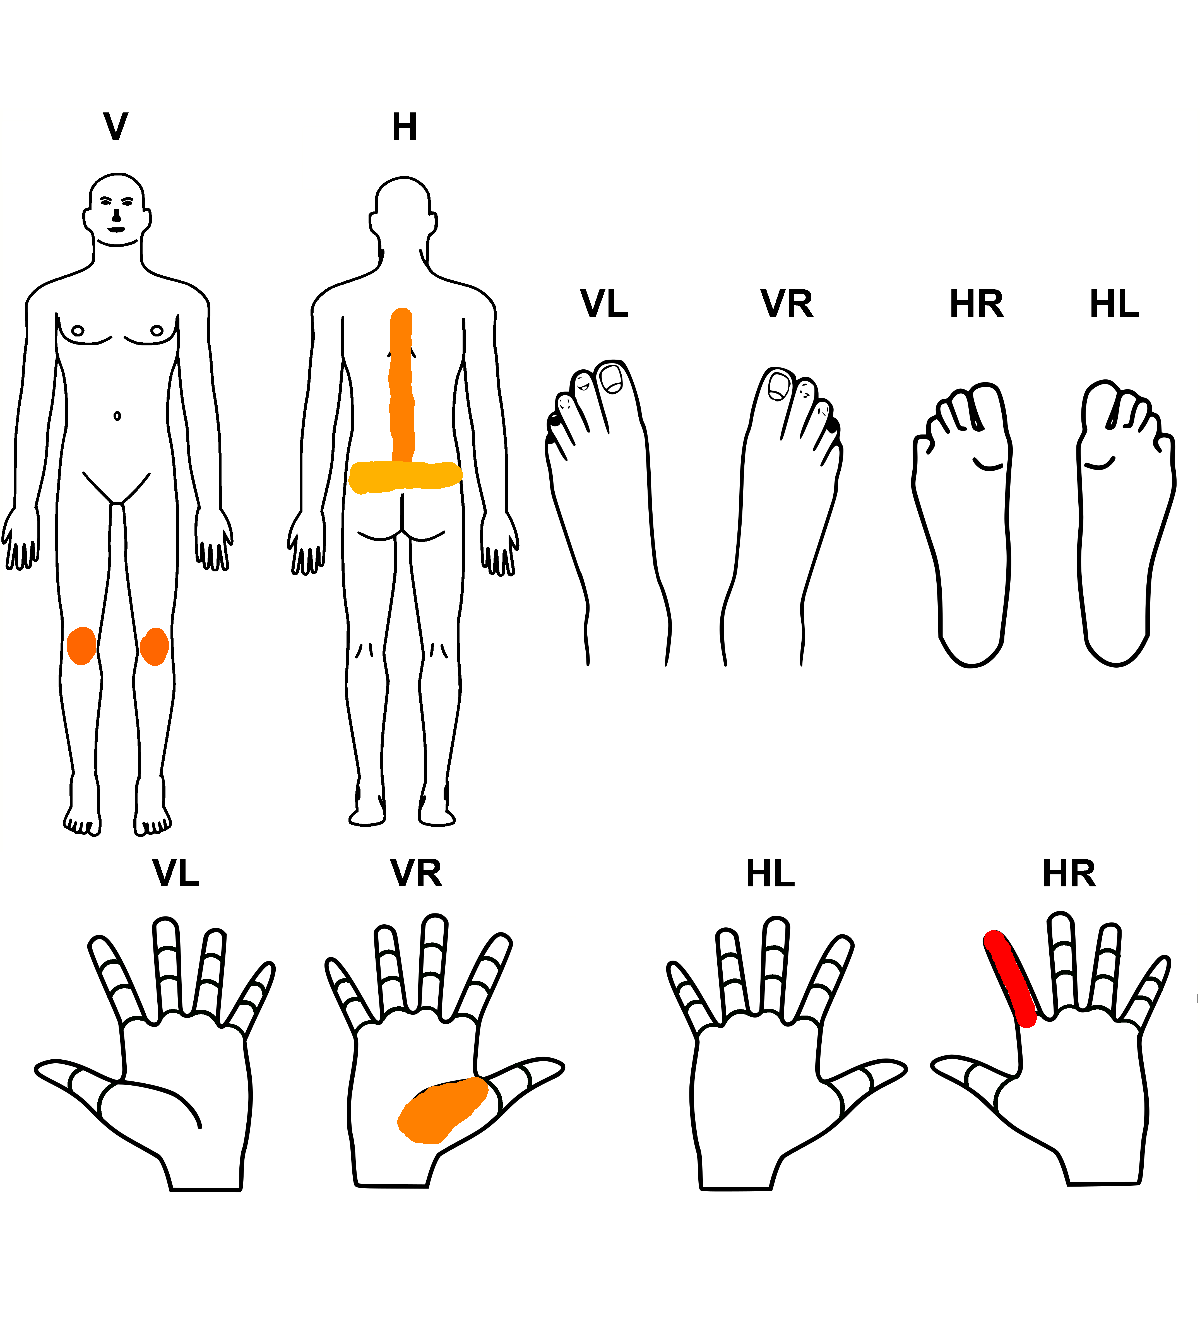
\includegraphics[width=0.5\textwidth]{images/pd.png}
    \caption{Example of a pain drawing representation used as input for machine learning.}
    \label{fig:my_image}
\end{figure}

The objective of the present work is to investigate whether pain drawings acquired from multiple clinical sources can be used for disease classification with neural networks. The current stage of the project focuses on three main questions: first, how heterogeneous pain drawing datasets can be standardized for training; second, how lightweight convolutional and fully connected neural architectures behave on small clinical datasets; and third, what the current experimental results imply for the next development stage of the dissertation work.

\chapter{Related Work}

The application of machine learning to medical image analysis has expanded rapidly over the last decade. Deep neural networks, in particular convolutional neural networks, have been widely adopted because they can learn hierarchical image representations directly from data instead of relying exclusively on handcrafted descriptors~\cite{litjens2017survey, lecun2015deep}. However, their success is typically strongest when sufficient labeled data are available and when acquisition conditions are relatively standardized.

Pain drawings differ from conventional medical images in two important ways. First, they are patient-generated rather than device-generated, meaning that they reflect subjective symptom localization instead of anatomical structure. Second, their diagnostic content is largely spatial and topological: clinically relevant information is encoded in where pain is marked, how extensively it is distributed, and whether it appears symmetrically or in characteristic body regions. Previous work, including the Pain2D framework, has shown that such representations can support disease differentiation and can therefore be treated as a meaningful computational modality rather than only as an illustrative patient note~\cite{emmert2018pain2d, wester2020pain}.

At the same time, pain drawing research faces challenges that are less prominent in large-scale image benchmarks. Datasets are often small, class distributions are strongly imbalanced, and acquisition protocols differ across hospitals or software platforms. These characteristics make model selection, preprocessing, and experimental design especially important. The present report therefore emphasizes not only predictive performance, but also the behavior and limitations of the implemented pipeline under realistic data constraints.

\chapter{Dataset Acquisition and Description}

\section{Conventional Pain Drawing Collection}

Historically, many pain drawings were collected on paper forms. Patients indicated painful areas on a printed body template, after which the forms were scanned and digitized for later inspection. Although this process preserves the anatomical location of reported pain, it introduces substantial variability. Differences in scan position, scaling, rotation, and image quality complicate any downstream analysis that assumes spatial correspondence across samples.

Another limitation of the conventional workflow is that it usually captures pain location only. Information about pain intensity is either absent or stored separately, which weakens the expressiveness of the final representation. For machine learning, this is problematic because the input should ideally preserve as much clinically relevant structure as possible while remaining standardized across patients.

\section{SeePain Data Collection}

To address these limitations, the \textit{SeePain} application was developed as a digital acquisition tool. Instead of paper-based annotation, patients directly mark pain regions on a standardized body template in a software environment. This removes scanning-related alignment errors and ensures that all collected drawings share the same underlying coordinate system.

An additional advantage of the digital workflow is that symptom intensity can be encoded visually through controlled color coding. As a result, SeePain data preserve not only the anatomical distribution of pain, but also a graded representation of severity. This richer input structure is expected to be especially useful for future models that explicitly incorporate color or intensity information.

\section{Datasets Description}

\begin{table}[h]
    \centering
    \begin{tabular}{|l|l|c|c|}
        \hline
        \textbf{Dataset Source} & \textbf{Classes} & \textbf{Samples per Class} & \textbf{Total Samples} \\
        \hline
        RWTH Aachen University & Others & 59 & \\
        & gHSD & 45 & \\
        & hEDS & 141 & 245 \\
        \hline
        MHH (IDANA Application) & Arthritis & 69 & \\
        & Kollagenose & 22 & \\
        & Polyarthritis & 359 & \\
        & Polymyalgia & 65 & \\
        & Sj\"ogren Syndrome & 38 & \\
        & Spondyloarthritis & 147 & \\
        & Unknown & 185 & 885 \\
        \hline
        MHH (SeePain Application) & Myositis & 4 & \\
        & Polymyalgia rheumatica & 7 & \\
        & Psoriasis-Arthritis & 17 & \\
        & Rheumatoide Arthritis & 35 & \\
        & Riesenzellarteriitis & 1 & \\
        & Sonstige & 31 & \\
        & axiale Spondyloarthritis & 10 & \\
        & Kollagenose & 12 & \\
        & nan & 7 & 124 \\
        \hline
        Munich Dataset & FSHD & 34 & \\
        & POMPE & 76 & \\
        & IBM & 16 & \\
        & SMA & 22 & 148 \\
        \hline
    \end{tabular}
    \caption{Overview of available datasets and class distributions. Both the IDANA and SeePain datasets originate from Hannover Medical School (MHH).}
    \label{tab:dataset_overview}
\end{table}

Three clinical sources contribute data to the current study: RWTH Aachen University, Hannover Medical School (MHH), and a Munich cohort. MHH contributes two distinct datasets because the data originate from two different acquisition systems, namely IDANA and SeePain. This is useful from a research perspective because it allows the investigation of both institution-level and platform-level variability.

The Aachen dataset contains three classes, namely Others, generalized hypermobility spectrum disorder (gHSD), and hypermobile Ehlers-Danlos syndrome (hEDS). The IDANA dataset is considerably larger and more heterogeneous, containing seven rheumatological categories. The SeePain dataset is smaller but clinically interesting because it was digitally acquired and contains disease classes from inflammatory and autoimmune contexts. The Munich dataset covers four neuromuscular disease categories.

Overall, the combined data are heterogeneous with respect to class counts, labeling granularity, and acquisition procedure. This heterogeneity is clinically realistic but computationally difficult. It introduces varying visual appearance, inter-disease similarity, and task-dependent complexity, all of which influence model behavior in the current experiments.

\chapter{Methodology and Pipeline}

\section{Overview}

The implemented pipeline is organized as a reproducible sequence of preprocessing, tensor generation, data loading, model training, evaluation, and plot generation. The main execution script loads a configuration file, optionally preprocesses a dataset, constructs training and validation loaders, initializes a selected model architecture, trains the model, evaluates it, and finally stores performance plots and confusion matrices.

\section{Data Loading and Conversion}

The project supports both direct image usage and reuse of preprocessed tensors. A separate preprocessing script converts raw PDF files to PNG format and copies image files into a unified directory structure. During model training, the main loader reads the dataset path from the configuration file and interprets each class folder as one label category. This folder-based organization provides a simple and extensible mechanism for switching between datasets without modifying the core training code.

For transparency and reproducibility, the implementation used for preprocessing, model definition, training, and evaluation is available in the associated project repository~\cite{rajgithub2026}.

\section{Data Preprocessing}

The preprocessing code performs the following operations before training:

\begin{itemize}
    \item all images are resized to a square resolution of \(1500 \times 1500\) pixels,
    \item images are converted to grayscale, resulting in a single-channel representation for the reported experiments,
    \item processed images are stored as PyTorch tensor files to accelerate repeated experiments,
    \item class balancing is performed by random undersampling before training.
\end{itemize}

The implemented preprocessing pipeline therefore prioritizes spatial standardization and controlled class balance. In the current experiments, class balancing is achieved by undersampling during preprocessing so that the training stage operates on balanced class subsets.

\section{Model Architectures}

Three architectures are currently represented in the generated experiments:

\begin{itemize}
    \item \textbf{SimpleCNNSmall:} a lightweight convolutional network with two convolutional layers, max pooling, one hidden fully connected layer, and dropout.
    \item \textbf{FCNNSmall:} a shallow fully connected baseline that flattens the entire image tensor and applies two hidden layers with dropout.
    \item \textbf{FCNNNet:} a deeper fully connected architecture with multiple dense layers and batch normalization.
\end{itemize}

In the fully connected setting, \textit{FCNNNet} was used as the larger baseline model. Since its training behavior suggested overfitting, a smaller fully connected alternative, namely \textit{FCNNSmall}, was introduced to examine whether reduced model capacity would generalize better. However, the smaller model performed worse in the current experiments. In addition, the source code already contains larger CNN and ResNet-based model definitions, although these were not part of the report figures generated for the present submission. Their availability indicates a clear pathway for extending the experimental study beyond the current baseline models.

\section{Training Setup}

The experimental settings used by the current pipeline are directly derived from the source code and configuration files:

\begin{itemize}
    \item optimizer: Adam,
    \item learning rate: \(0.001\),
    \item batch size: \(16\),
    \item number of epochs: \(50\),
    \item train/validation split: \(75\% / 25\%\),
    \item loss function: cross-entropy loss.
\end{itemize}

Training and validation accuracy as well as loss are recorded at every epoch. After training, the model is evaluated again on the validation split, and the predictions are used to generate a normalized confusion matrix.

\section{Evaluation Metrics}

The following outputs are used to analyze model behavior:

\begin{itemize}
    \item training loss,
    \item validation loss,
    \item training accuracy,
    \item validation accuracy,
    \item row-normalized confusion matrices.
\end{itemize}

A model may achieve a seemingly acceptable validation score while still collapsing to one dominant class. The row-normalized matrices therefore provide a better view of class-wise recall and failure modes.

\chapter{Experiments}

\section{Experimental Design}

The experiments reported here were designed as a comparative baseline study across datasets with different clinical origin and class structure. Each experiment uses the same training code and the same high-level optimization setup, allowing the observed differences to be attributed primarily to dataset characteristics and model architecture.

Because several original datasets contain extreme imbalance or very small categories, the current experimental setup uses reduced classification tasks for some cohorts. The class filtering is defined in the configuration files and is applied before preprocessing and training. After filtering, the retained classes are balanced by undersampling so that each class contributes equally during training. This decision was necessary to obtain trainable subsets while keeping the first evaluation stage computationally manageable.

\section{Tasks Included in the Present Report}

\begin{table}[H]
    \centering
    \begin{tabular}{|>{\raggedright\arraybackslash}p{3.5cm}|>{\raggedright\arraybackslash}p{4cm}|>{\raggedright\arraybackslash}p{5cm}|}
        \hline
        \textbf{Dataset} & \textbf{Reported Task} & \textbf{Classes Used in Experiment} \\
        \hline
        Aachen & 3-class classification & Others, gHSD, hEDS \\
        \hline
        MHH SeePain & 2-class classification & Psoriasis-Arthritis, Rheumatoide Arthritis \\
        \hline
        MHH IDANA & 4-class classification & Arthritis, Polyarthritis, Polymyalgia, Spondyloarthritis \\
        \hline
        Munich & 2-class classification & FSHD, POMPE \\
        \hline
    \end{tabular}
    \caption{Classification tasks represented by the generated result figures.}
    \label{tab:experimental_tasks}
\end{table}

This staged strategy is methodologically justified. The primary purpose of the current phase is not yet to maximize headline accuracy, but to understand whether the implemented pipeline can learn clinically meaningful structure and which architectures remain stable under limited-data conditions.

\chapter{Results}

\section{Aachen Dataset}

The Aachen experiment is the most informative multi-class result in the current report because all three diagnostic groups are retained. The deeper fully connected model (\textit{FCNNNet}) performs best among the tested architectures in the sense that it captures the dominant hEDS pattern strongly, with row-normalized recalls of approximately 0.93 for one class and 0.88 for another. However, the same confusion matrix also shows weak separation for one class, indicating that the model is not yet clinically reliable for balanced three-class discrimination.

The shallow fully connected baseline (\textit{FCNNSmall}) collapses almost completely to one prediction column, which means that it effectively learns a majority-class solution rather than a discriminative representation. The lightweight convolutional model (\textit{SimpleCNNSmall}) behaves more evenly and distributes predictions across classes, but its confusion matrix still reveals substantial inter-class mixing. This suggests that the Aachen task is learnable to some extent, but the current baselines are not yet robust enough to separate all three diagnoses consistently.

\begin{figure}[H]
    \centering
    \begin{subfigure}{0.3\textwidth}
        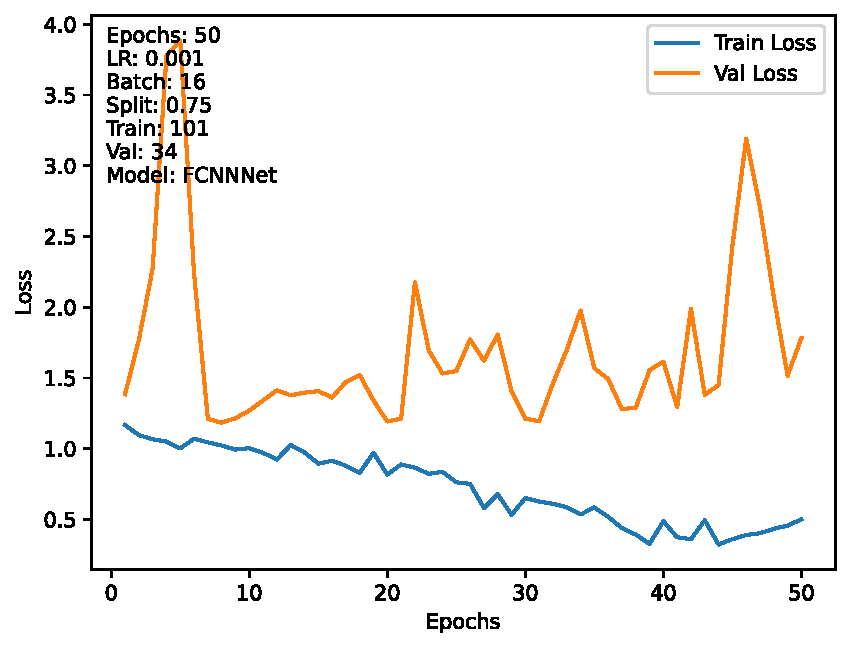
\includegraphics[width=\linewidth]{images/aachen_num_classes_3_FCNNNet_loss.pdf}
        \caption{FCNNNet - Loss}
    \end{subfigure}
    \hfill
    \begin{subfigure}{0.3\textwidth}
        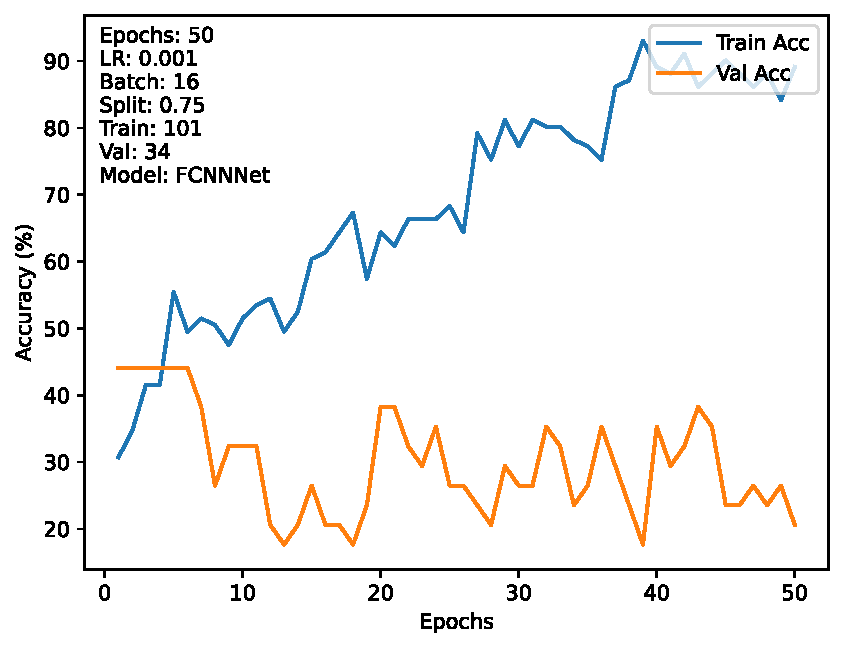
\includegraphics[width=\linewidth]{images/aachen_num_classes_3_FCNNNet_accuracy.pdf}
        \caption{FCNNNet - Accuracy}
    \end{subfigure}
    \hfill
    \begin{subfigure}{0.3\textwidth}
        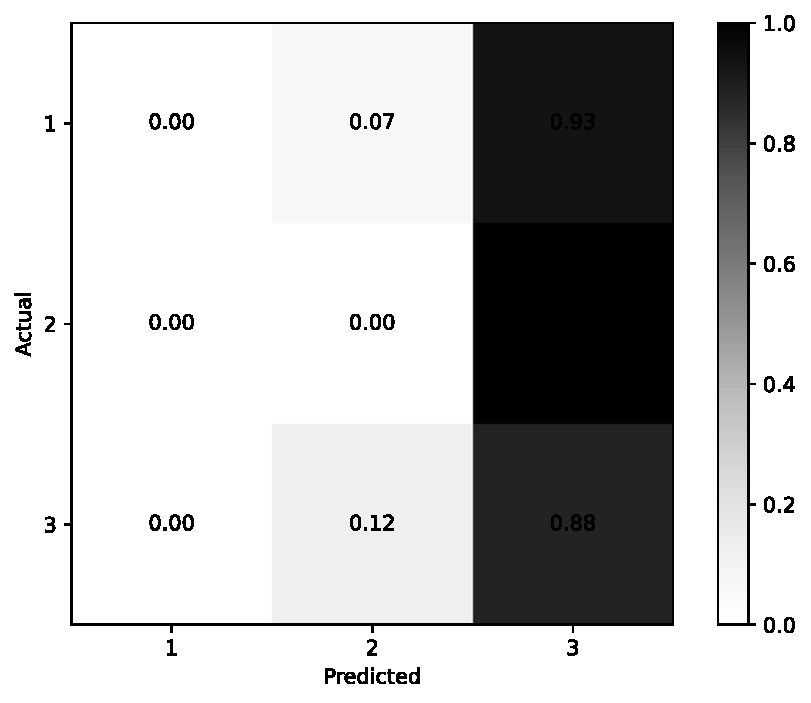
\includegraphics[width=\linewidth]{images/aachen_num_classes_3_FCNNNet_confusion_matrix.pdf}
        \caption{FCNNNet - Confusion Matrix}
    \end{subfigure}

    \vspace{0.3cm}

    \begin{subfigure}{0.3\textwidth}
        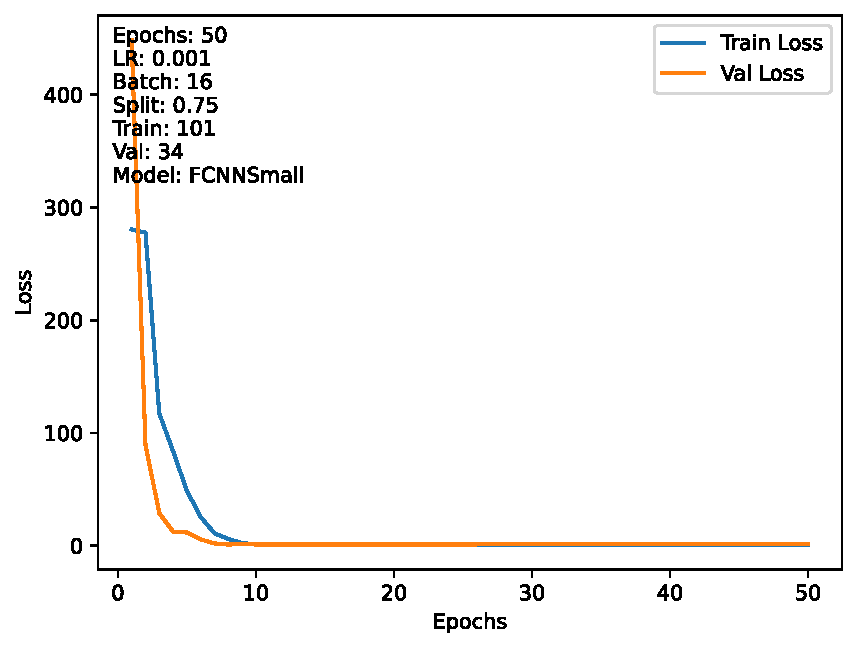
\includegraphics[width=\linewidth]{images/aachen_num_classes_3_FCNNSmall_loss.pdf}
        \caption{FCNNSmall - Loss}
    \end{subfigure}
    \hfill
    \begin{subfigure}{0.3\textwidth}
        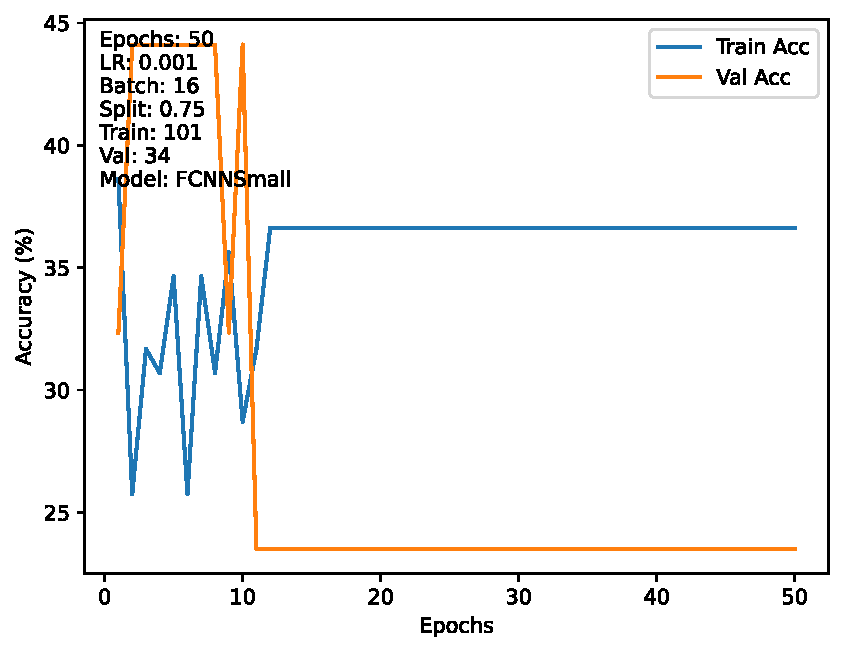
\includegraphics[width=\linewidth]{images/aachen_num_classes_3_FCNNSmall_accuracy.pdf}
        \caption{FCNNSmall - Accuracy}
    \end{subfigure}
    \hfill
    \begin{subfigure}{0.3\textwidth}
        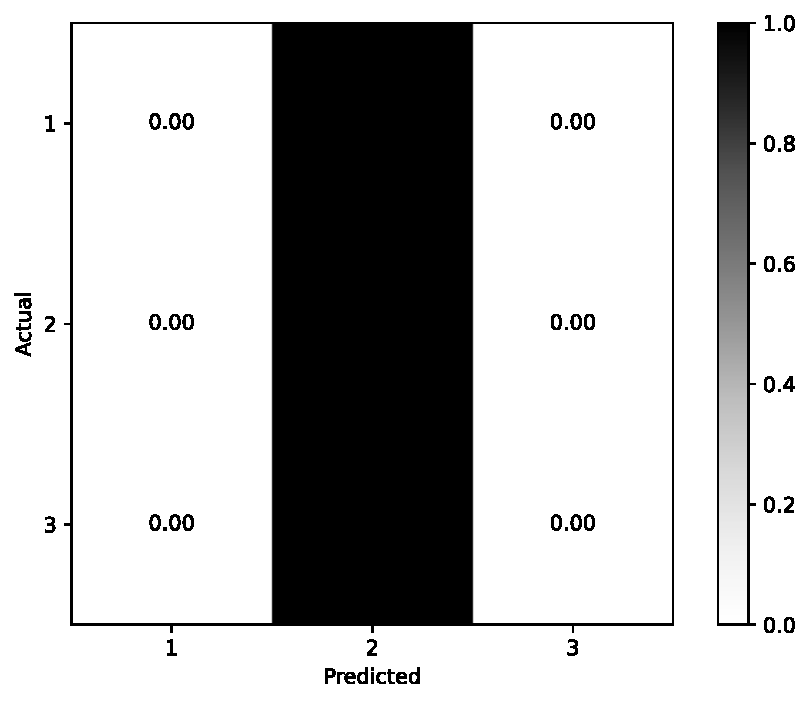
\includegraphics[width=\linewidth]{images/aachen_num_classes_3_FCNNSmall_confusion_matrix.pdf}
        \caption{FCNNSmall - Confusion Matrix}
    \end{subfigure}

    \vspace{0.3cm}

    \begin{subfigure}{0.3\textwidth}
        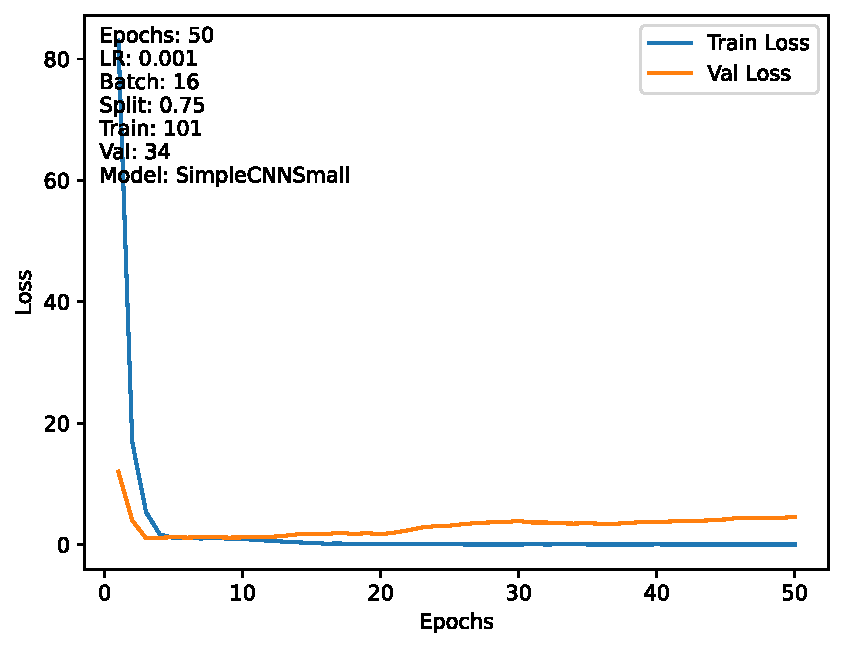
\includegraphics[width=\linewidth]{images/aachen_num_classes_3_SimpleCNNSmall_loss.pdf}
        \caption{SimpleCNNSmall - Loss}
    \end{subfigure}
    \hfill
    \begin{subfigure}{0.3\textwidth}
        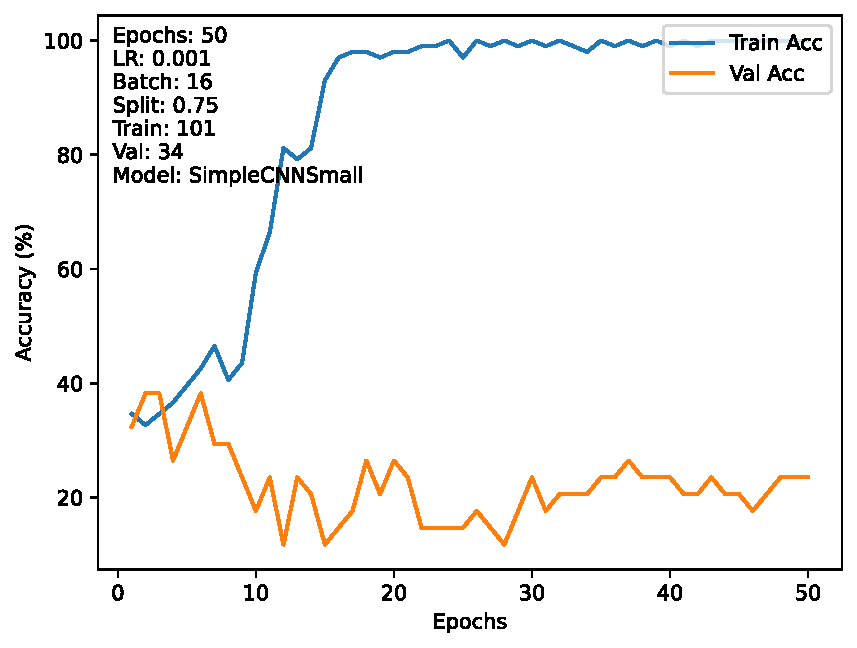
\includegraphics[width=\linewidth]{images/aachen_num_classes_3_SimpleCNNSmall_accuracy.pdf}
        \caption{SimpleCNNSmall - Accuracy}
    \end{subfigure}
    \hfill
    \begin{subfigure}{0.3\textwidth}
        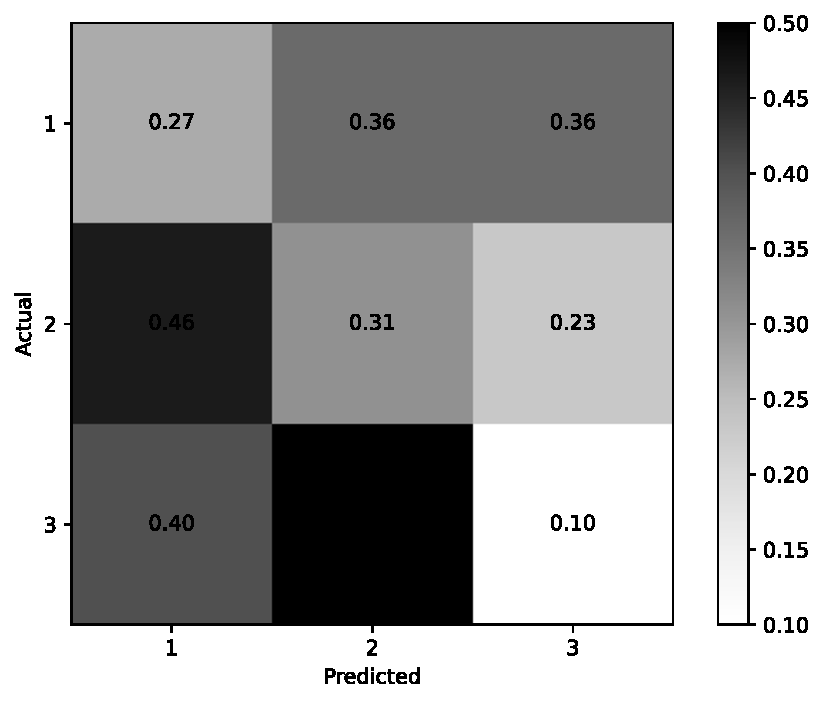
\includegraphics[width=\linewidth]{images/aachen_num_classes_3_SimpleCNNSmall_confusion_matrix.pdf}
        \caption{SimpleCNNSmall - Confusion Matrix}
    \end{subfigure}

    \caption{Model comparison on the Aachen dataset.}
\end{figure}

\clearpage
\section{MHH SeePain Dataset}

The binary SeePain experiment is based on the two classes with sufficient data after filtering, namely Psoriasis-Arthritis and Rheumatoide Arthritis. Despite the simplified label space, the reported confusion matrices indicate a degenerate behavior: the tested models predict only one class for all validation samples. In row-normalized form, this appears as 0.00 in the first prediction column and 1.00 in the second prediction column for both rows.

This result is important because it shows that digital acquisition alone does not automatically solve the learning problem. The current binary task remains challenging for the present baselines even after class filtering and preprocessing. At the same time, the task remains promising because the input standardization achieved by SeePain provides higher-quality pain drawings than conventional collection procedures. Therefore, better results may reasonably be expected once a larger SeePain dataset becomes available. For future machine learning analysis, a practical target would be at least a few hundred samples overall, and ideally on the order of 100 to 200 pain drawings per class, so that model training and validation can be carried out more reliably.

\begin{figure}[H]
    \centering
    \begin{subfigure}{0.3\textwidth}
        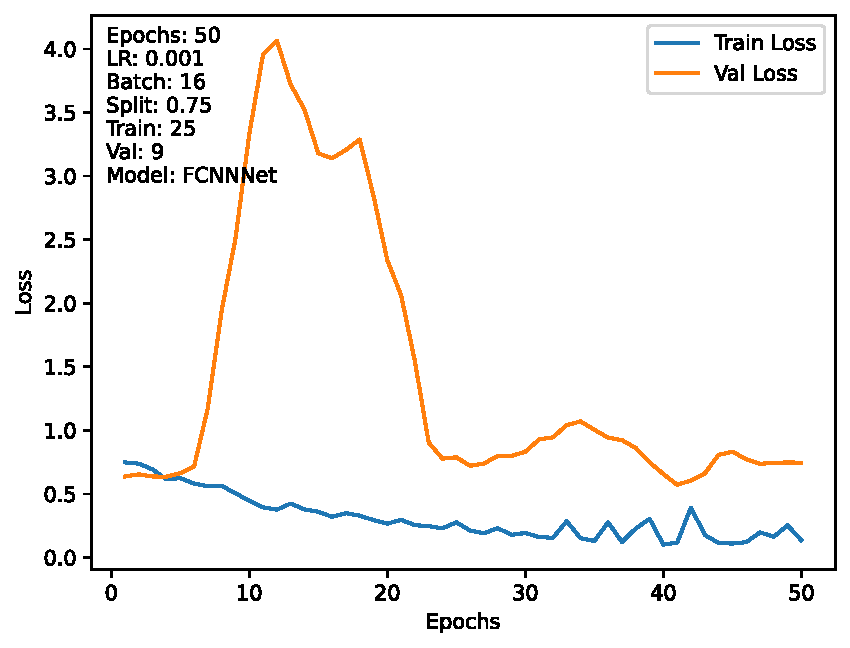
\includegraphics[width=\linewidth]{images/mhh_seepain_num_classes_2_FCNNNet_loss.pdf}
        \caption{FCNNNet - Loss}
    \end{subfigure}
    \hfill
    \begin{subfigure}{0.3\textwidth}
        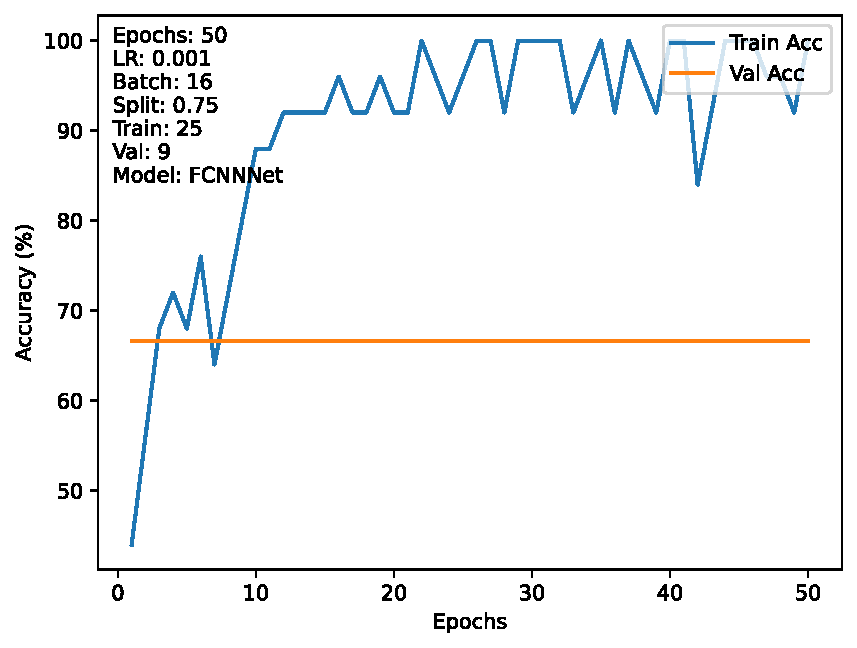
\includegraphics[width=\linewidth]{images/mhh_seepain_num_classes_2_FCNNNet_accuracy.pdf}
        \caption{FCNNNet - Accuracy}
    \end{subfigure}
    \hfill
    \begin{subfigure}{0.3\textwidth}
        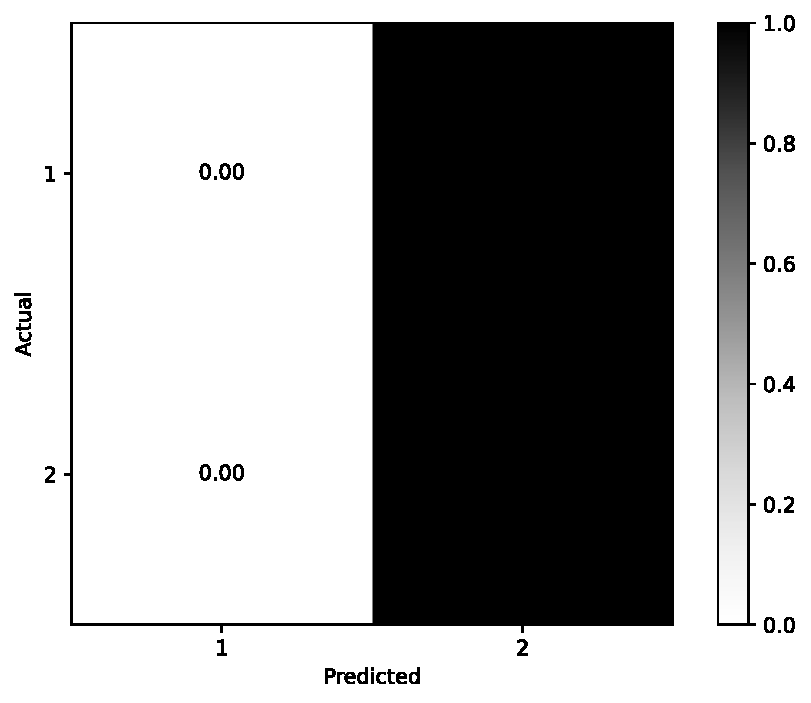
\includegraphics[width=\linewidth]{images/mhh_seepain_num_classes_2_FCNNNet_confusion_matrix.pdf}
        \caption{FCNNNet - Confusion Matrix}
    \end{subfigure}

    \vspace{0.3cm}

    \begin{subfigure}{0.3\textwidth}
        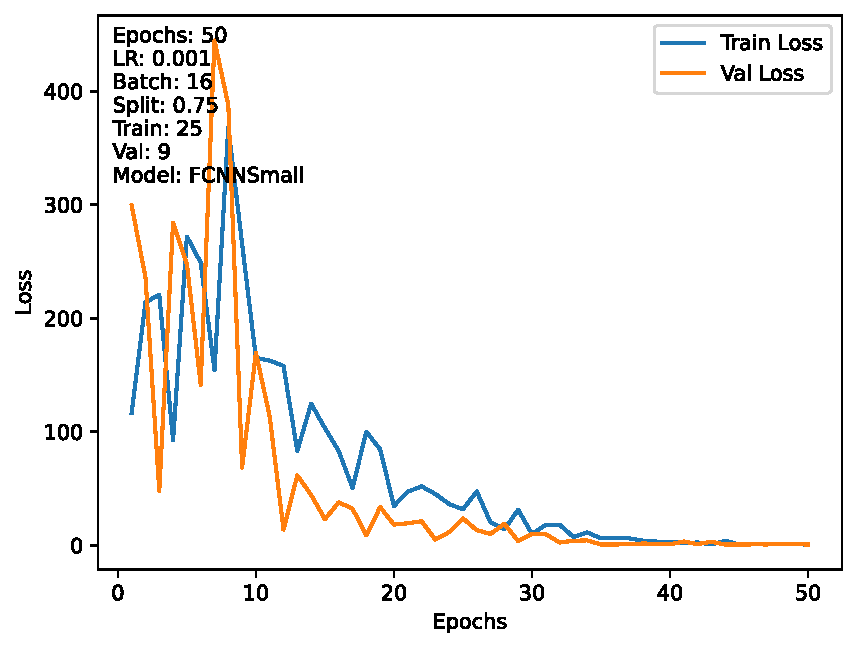
\includegraphics[width=\linewidth]{images/mhh_seepain_num_classes_2_FCNNSmall_loss.pdf}
        \caption{FCNNSmall - Loss}
    \end{subfigure}
    \hfill
    \begin{subfigure}{0.3\textwidth}
        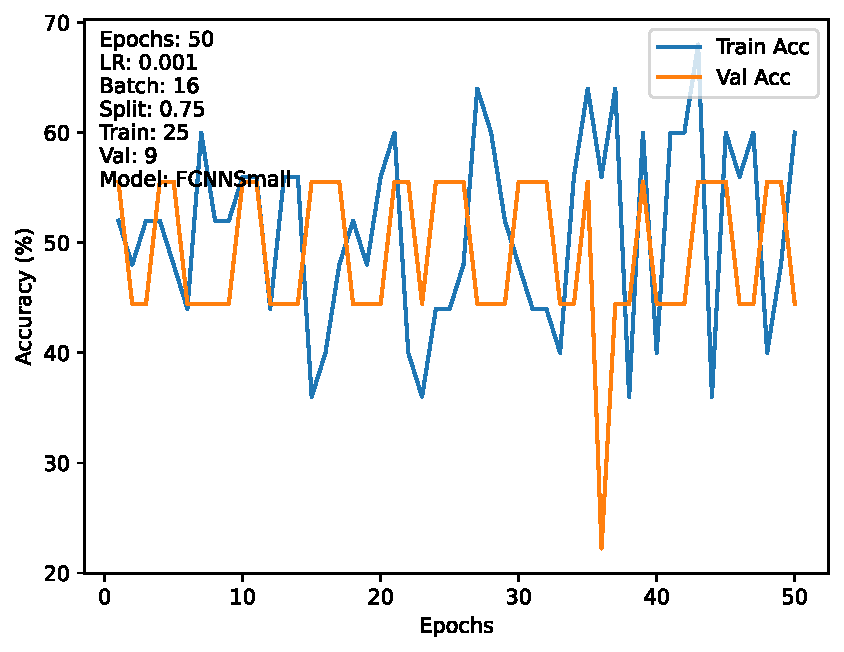
\includegraphics[width=\linewidth]{images/mhh_seepain_num_classes_2_FCNNSmall_accuracy.pdf}
        \caption{FCNNSmall - Accuracy}
    \end{subfigure}
    \hfill
    \begin{subfigure}{0.3\textwidth}
        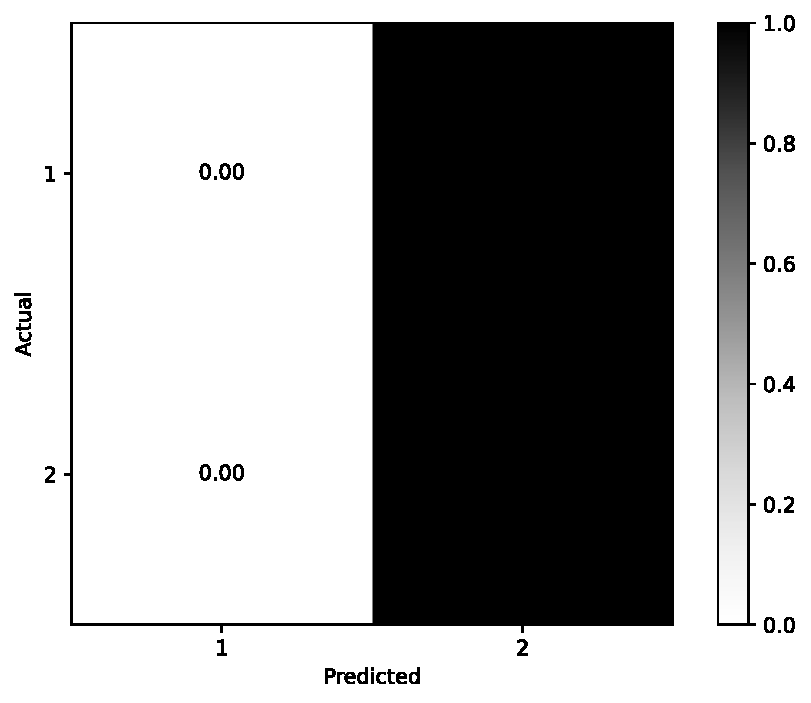
\includegraphics[width=\linewidth]{images/mhh_seepain_num_classes_2_FCNNSmall_confusion_matrix.pdf}
        \caption{FCNNSmall - Confusion Matrix}
    \end{subfigure}

    \vspace{0.3cm}

    \begin{subfigure}{0.3\textwidth}
        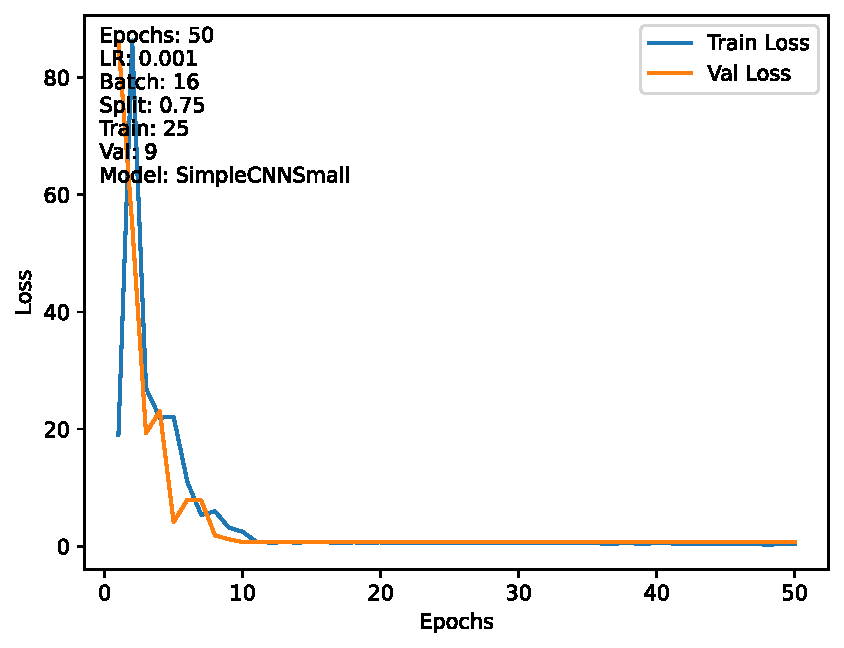
\includegraphics[width=\linewidth]{images/mhh_seepain_num_classes_2_SimpleCNNSmall_loss.pdf}
        \caption{SimpleCNNSmall - Loss}
    \end{subfigure}
    \hfill
    \begin{subfigure}{0.3\textwidth}
        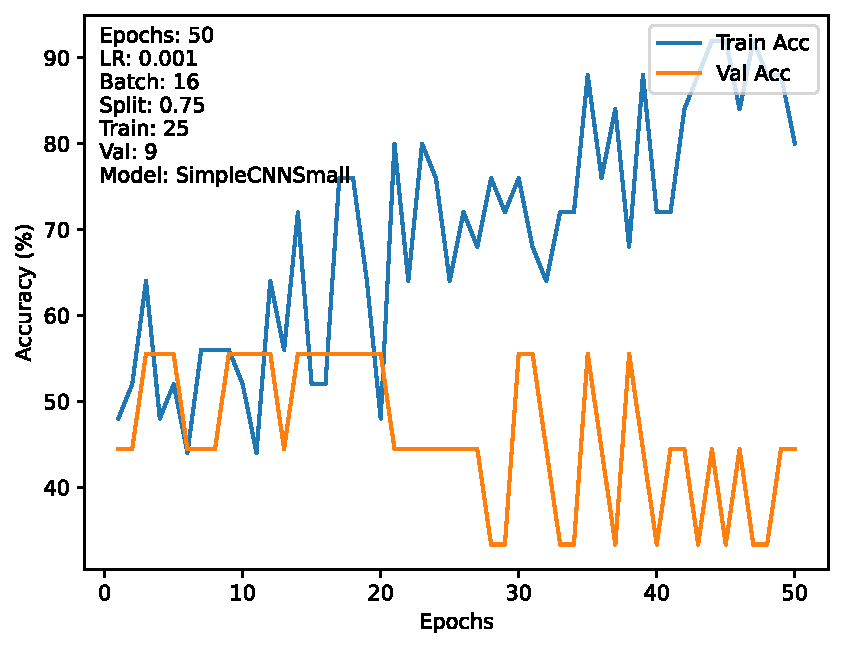
\includegraphics[width=\linewidth]{images/mhh_seepain_num_classes_2_SimpleCNNSmall_accuracy.pdf}
        \caption{SimpleCNNSmall - Accuracy}
    \end{subfigure}
    \hfill
    \begin{subfigure}{0.3\textwidth}
        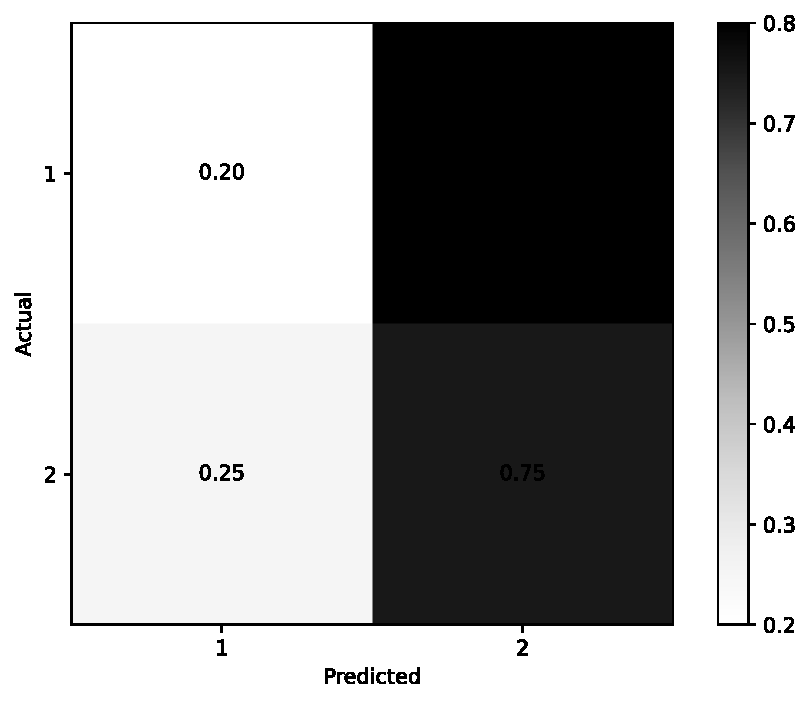
\includegraphics[width=\linewidth]{images/mhh_seepain_num_classes_2_SimpleCNNSmall_confusion_matrix.pdf}
        \caption{SimpleCNNSmall - Confusion Matrix}
    \end{subfigure}

    \caption{Model comparison on the MHH SeePain binary task.}
\end{figure}

\clearpage
\section{MHH IDANA Dataset}

Among the MHH experiments, the IDANA subset provides the clearest evidence that the models can learn something meaningful while still showing strong prediction bias. The best result again comes from \textit{FCNNNet}. Its confusion matrix shows that one class is identified perfectly and two additional classes achieve high recall values around 0.95 and 0.89, but the first class is still almost entirely confused with another category. This indicates partial structure learning rather than full multi-class discrimination. At the same time, the IDANA data appear to have been collected with relatively poor consistency and quality, which is likely one of the reasons the neural networks struggle to identify stable diagnostic patterns.

Both \textit{FCNNSmall} and \textit{SimpleCNNSmall} collapse to a single class in this setting, which is visible from their confusion matrices containing 1.00 in the same prediction column across all rows. The comparison therefore suggests that greater model capacity helps on the more complex IDANA task, but capacity alone is not sufficient to resolve the visual overlap between diagnostic patterns. The poor collection quality of the IDANA data is also an important limitation and may directly reduce the ability of the models to learn reliable structure from these samples.

\begin{figure}[H]
    \centering
    \begin{subfigure}{0.3\textwidth}
        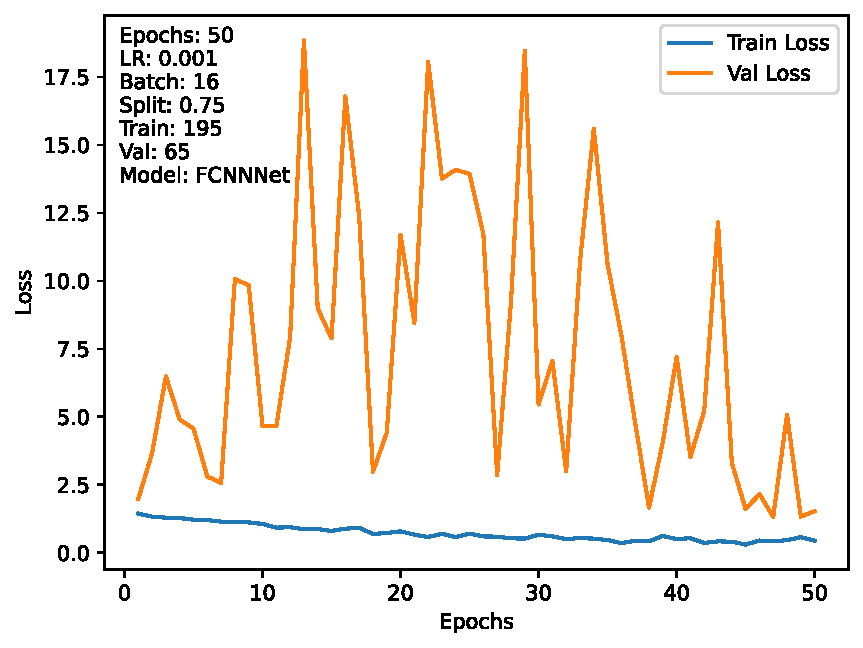
\includegraphics[width=\linewidth]{images/mhh_idana_num_classes_4_FCNNNet_loss.pdf}
        \caption{FCNNNet - Loss}
    \end{subfigure}
    \hfill
    \begin{subfigure}{0.3\textwidth}
        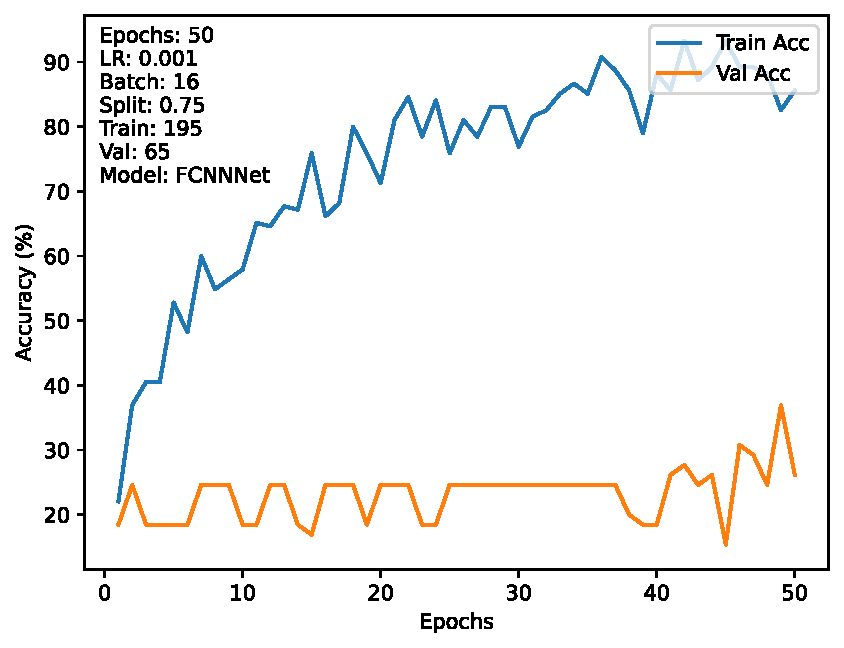
\includegraphics[width=\linewidth]{images/mhh_idana_num_classes_4_FCNNNet_accuracy.pdf}
        \caption{FCNNNet - Accuracy}
    \end{subfigure}
    \hfill
    \begin{subfigure}{0.3\textwidth}
        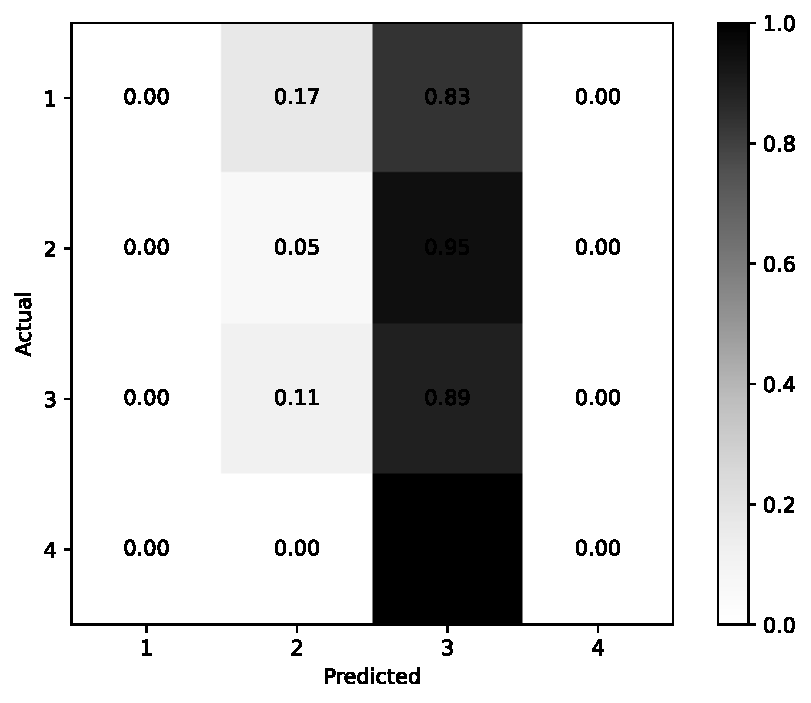
\includegraphics[width=\linewidth]{images/mhh_idana_num_classes_4_FCNNNet_confusion_matrix.pdf}
        \caption{FCNNNet - Confusion Matrix}
    \end{subfigure}

    \vspace{0.3cm}

    \begin{subfigure}{0.3\textwidth}
        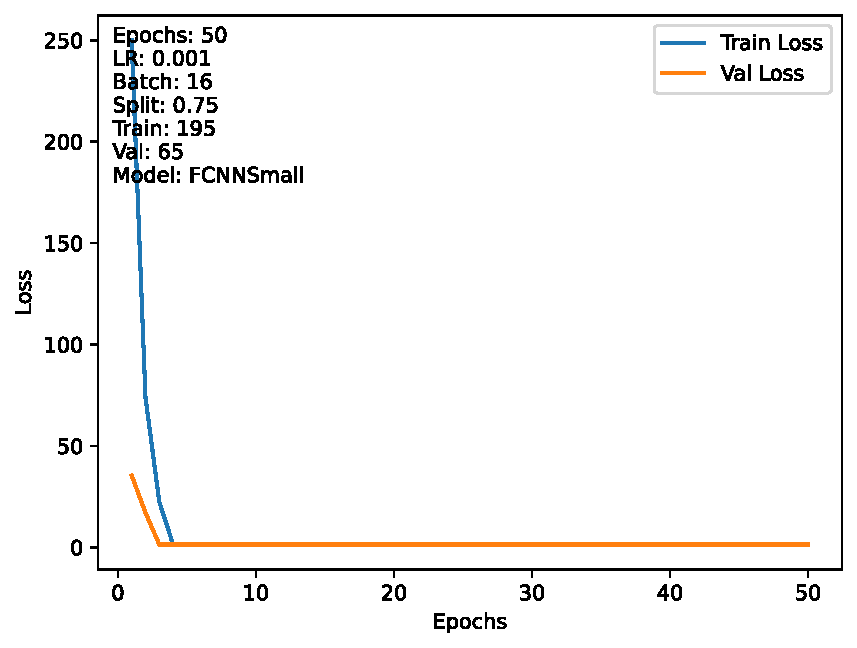
\includegraphics[width=\linewidth]{images/mhh_idana_num_classes_4_FCNNSmall_loss.pdf}
        \caption{FCNNSmall - Loss}
    \end{subfigure}
    \hfill
    \begin{subfigure}{0.3\textwidth}
        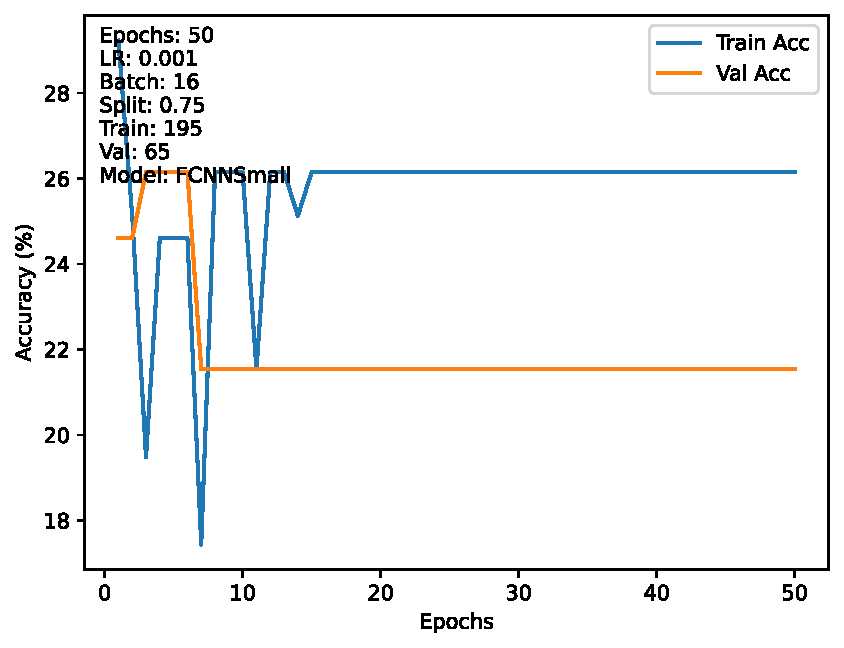
\includegraphics[width=\linewidth]{images/mhh_idana_num_classes_4_FCNNSmall_accuracy.pdf}
        \caption{FCNNSmall - Accuracy}
    \end{subfigure}
    \hfill
    \begin{subfigure}{0.3\textwidth}
        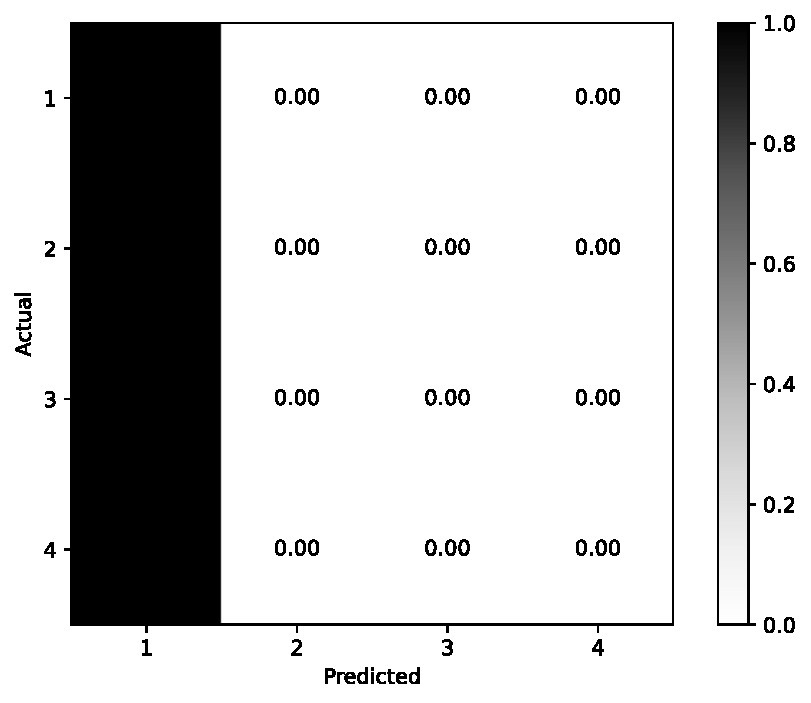
\includegraphics[width=\linewidth]{images/mhh_idana_num_classes_4_FCNNSmall_confusion_matrix.pdf}
        \caption{FCNNSmall - Confusion Matrix}
    \end{subfigure}

    \vspace{0.3cm}

    \begin{subfigure}{0.3\textwidth}
        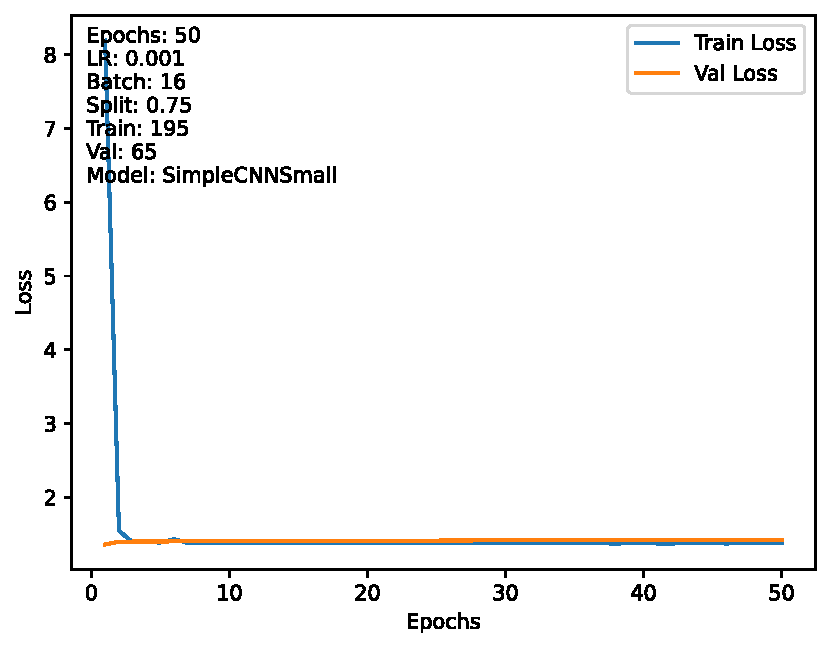
\includegraphics[width=\linewidth]{images/mhh_idana_num_classes_4_SimpleCNNSmall_loss.pdf}
        \caption{SimpleCNNSmall - Loss}
    \end{subfigure}
    \hfill
    \begin{subfigure}{0.3\textwidth}
        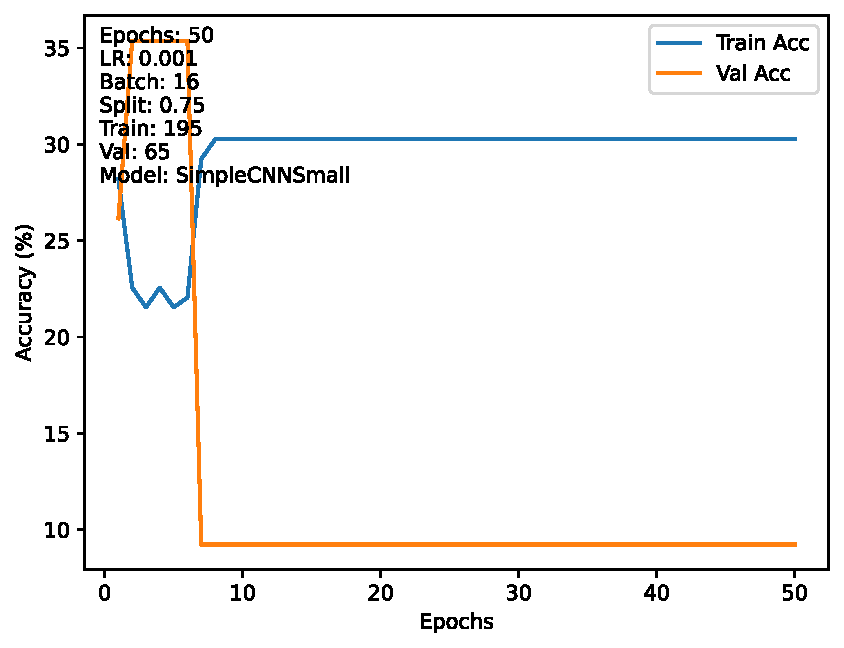
\includegraphics[width=\linewidth]{images/mhh_idana_num_classes_4_SimpleCNNSmall_accuracy.pdf}
        \caption{SimpleCNNSmall - Accuracy}
    \end{subfigure}
    \hfill
    \begin{subfigure}{0.3\textwidth}
        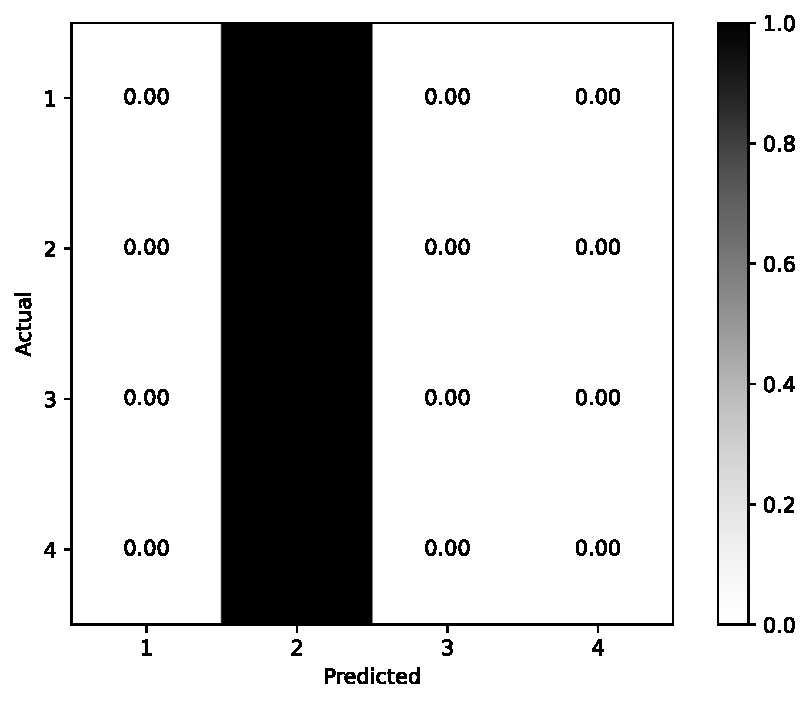
\includegraphics[width=\linewidth]{images/mhh_idana_num_classes_4_SimpleCNNSmall_confusion_matrix.pdf}
        \caption{SimpleCNNSmall - Confusion Matrix}
    \end{subfigure}

    \caption{Model comparison on the MHH IDANA 4-class task.}
\end{figure}

\section{Munich Dataset}

The Munich binary task shows behavior similar to the SeePain binary experiment. The evaluated models collapse to the same prediction column for all validation samples, indicating that they primarily learn the dominant class rather than the distinction between FSHD and Pompe disease. This is a useful negative result because it highlights that the current preprocessing and architecture choices are not yet sufficient for reliable discrimination, even when the class space is reduced to two labels.

Taken together, the Munich and SeePain results show that binary classification does not automatically become easier when the underlying dataset remains small. For this type of clinical data, class count alone is therefore not a good proxy for task difficulty.

\begin{figure}[H]
    \centering
    \begin{subfigure}{0.3\textwidth}
        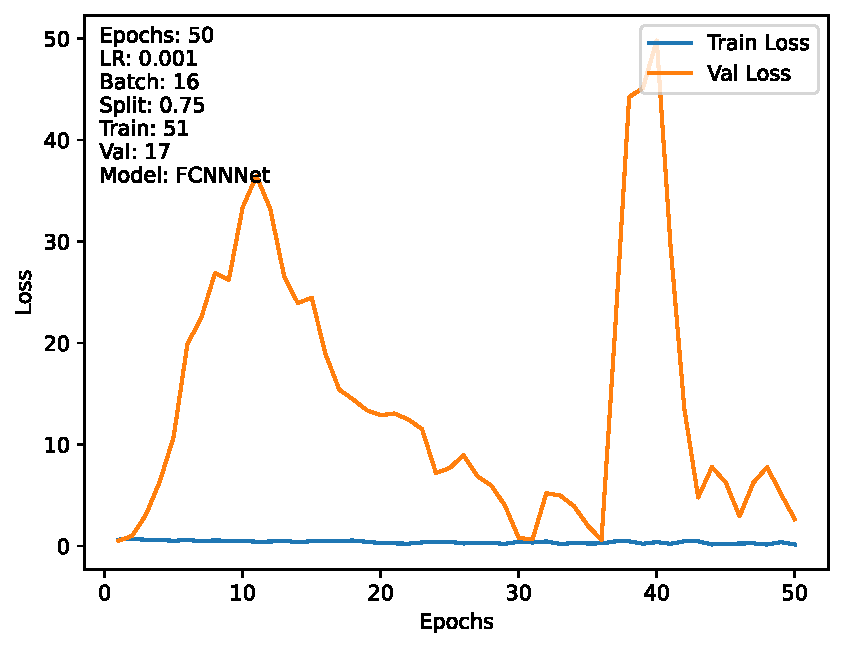
\includegraphics[width=\linewidth]{images/munich_num_classes_2_FCNNNet_loss.pdf}
        \caption{FCNNNet - Loss}
    \end{subfigure}
    \hfill
    \begin{subfigure}{0.3\textwidth}
        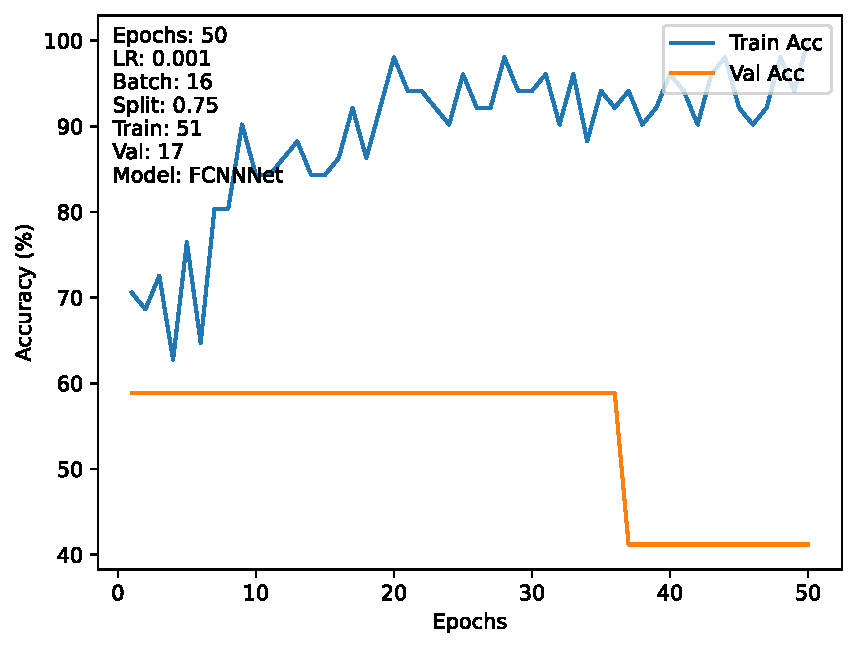
\includegraphics[width=\linewidth]{images/munich_num_classes_2_FCNNNet_accuracy.pdf}
        \caption{FCNNNet - Accuracy}
    \end{subfigure}
    \hfill
    \begin{subfigure}{0.3\textwidth}
        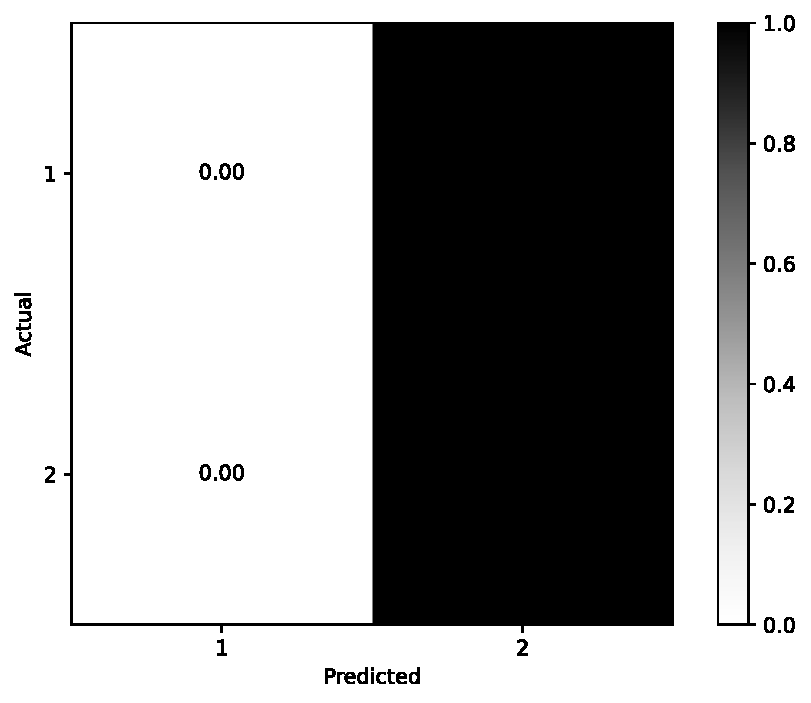
\includegraphics[width=\linewidth]{images/munich_num_classes_2_FCNNNet_confusion_matrix.pdf}
        \caption{FCNNNet - Confusion Matrix}
    \end{subfigure}

    \vspace{0.3cm}

    \begin{subfigure}{0.3\textwidth}
        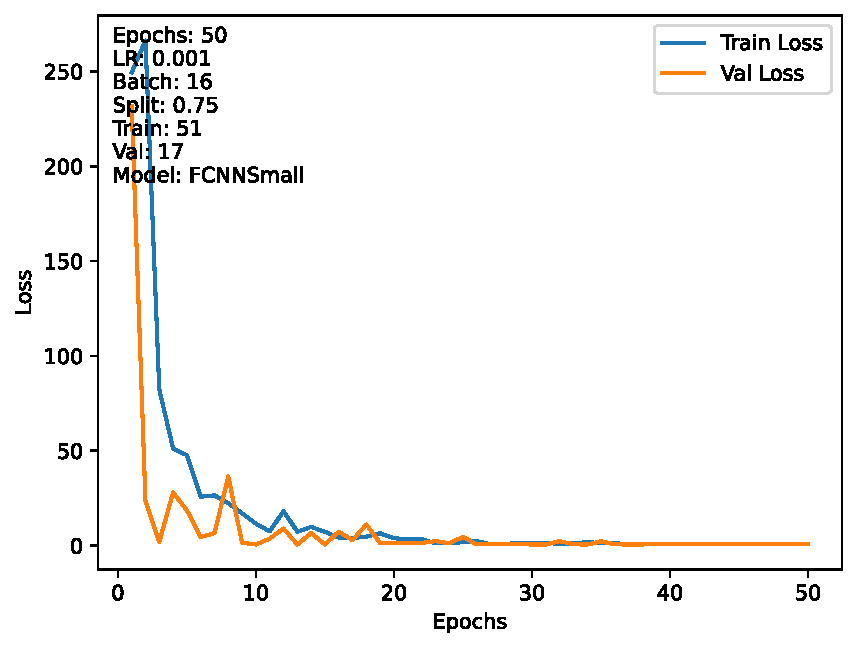
\includegraphics[width=\linewidth]{images/munich_num_classes_2_FCNNSmall_loss.pdf}
        \caption{FCNNSmall - Loss}
    \end{subfigure}
    \hfill
    \begin{subfigure}{0.3\textwidth}
        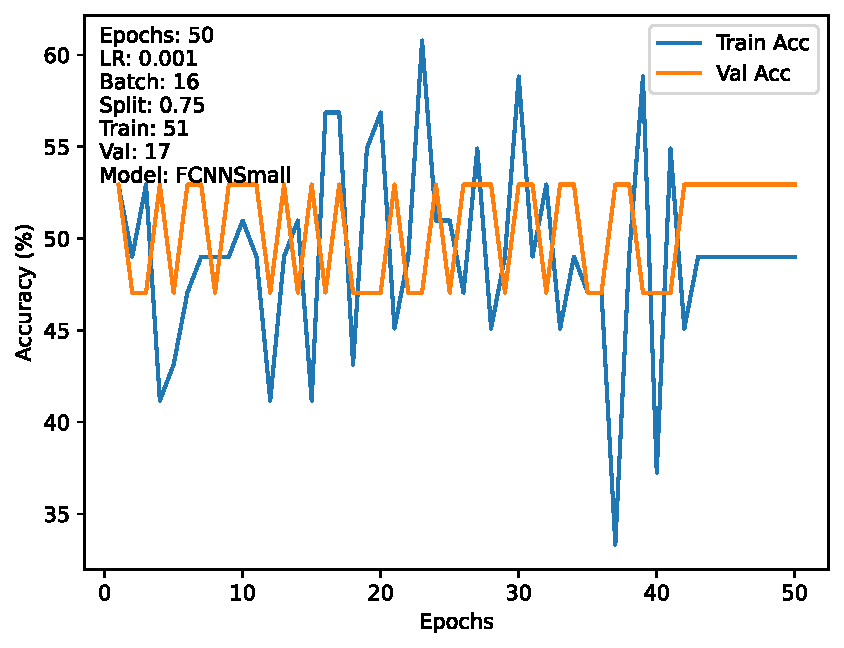
\includegraphics[width=\linewidth]{images/munich_num_classes_2_FCNNSmall_accuracy.pdf}
        \caption{FCNNSmall - Accuracy}
    \end{subfigure}
    \hfill
    \begin{subfigure}{0.3\textwidth}
        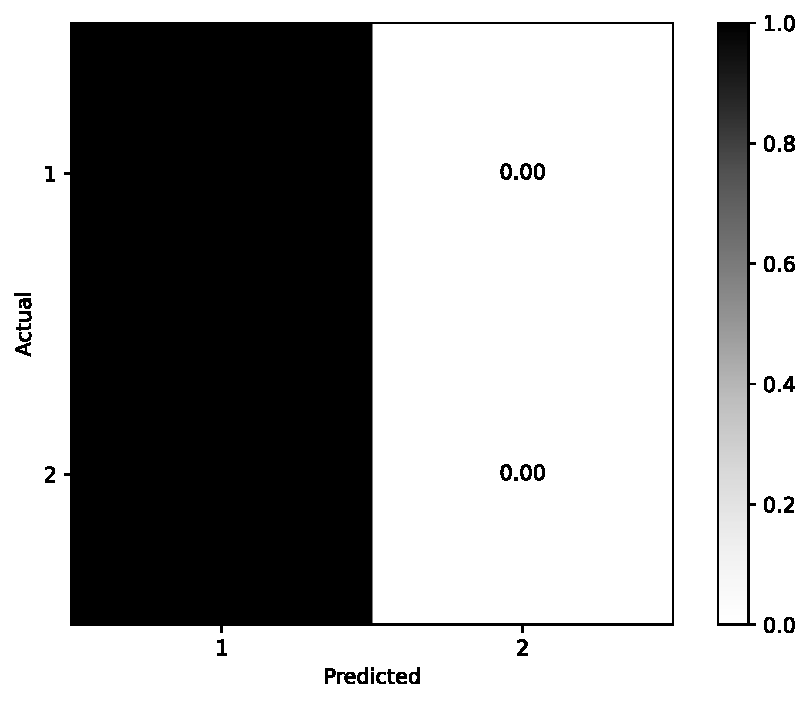
\includegraphics[width=\linewidth]{images/munich_num_classes_2_FCNNSmall_confusion_matrix.pdf}
        \caption{FCNNSmall - Confusion Matrix}
    \end{subfigure}

    \vspace{0.3cm}

    \begin{subfigure}{0.3\textwidth}
        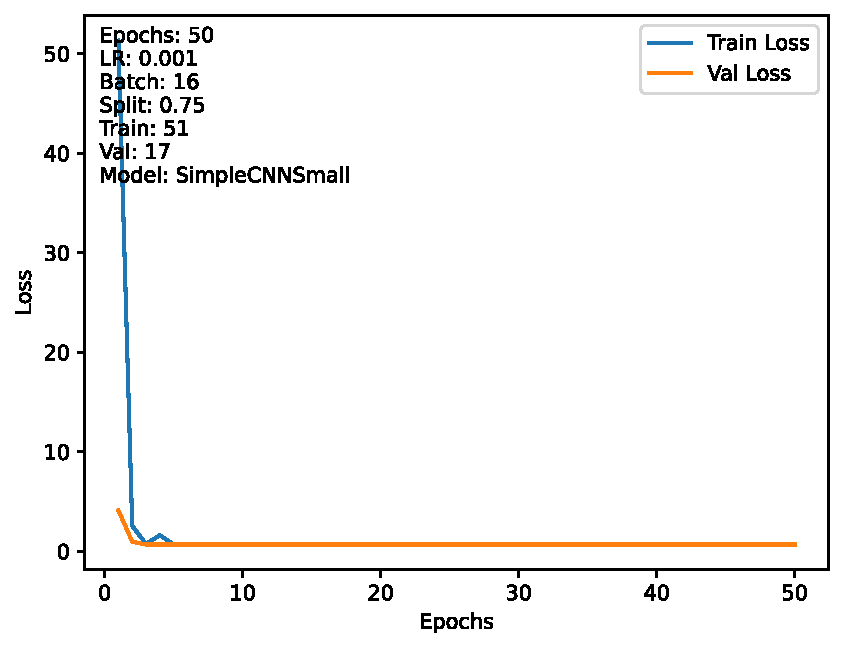
\includegraphics[width=\linewidth]{images/munich_num_classes_2_SimpleCNNSmall_loss.pdf}
        \caption{SimpleCNNSmall - Loss}
    \end{subfigure}
    \hfill
    \begin{subfigure}{0.3\textwidth}
        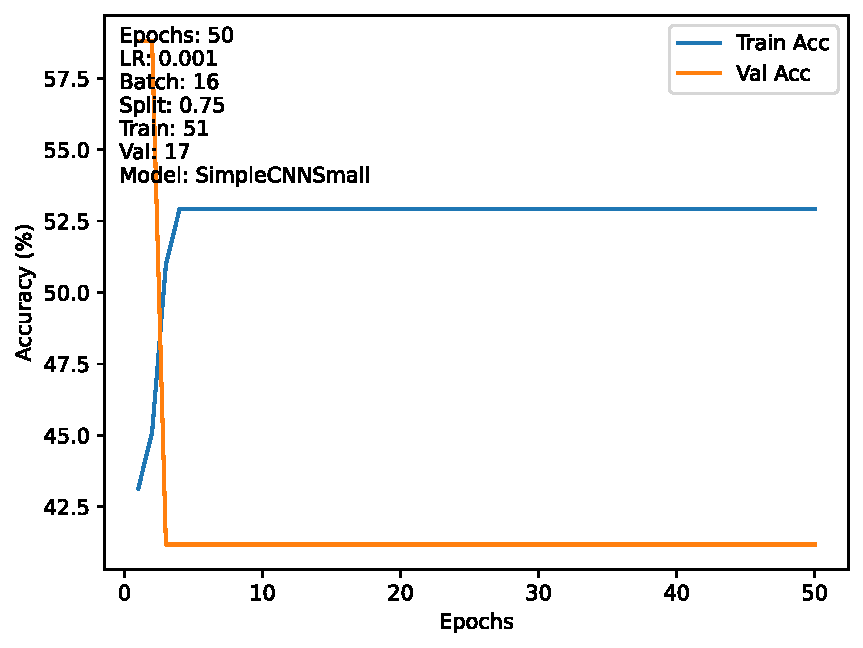
\includegraphics[width=\linewidth]{images/munich_num_classes_2_SimpleCNNSmall_accuracy.pdf}
        \caption{SimpleCNNSmall - Accuracy}
    \end{subfigure}
    \hfill
    \begin{subfigure}{0.3\textwidth}
        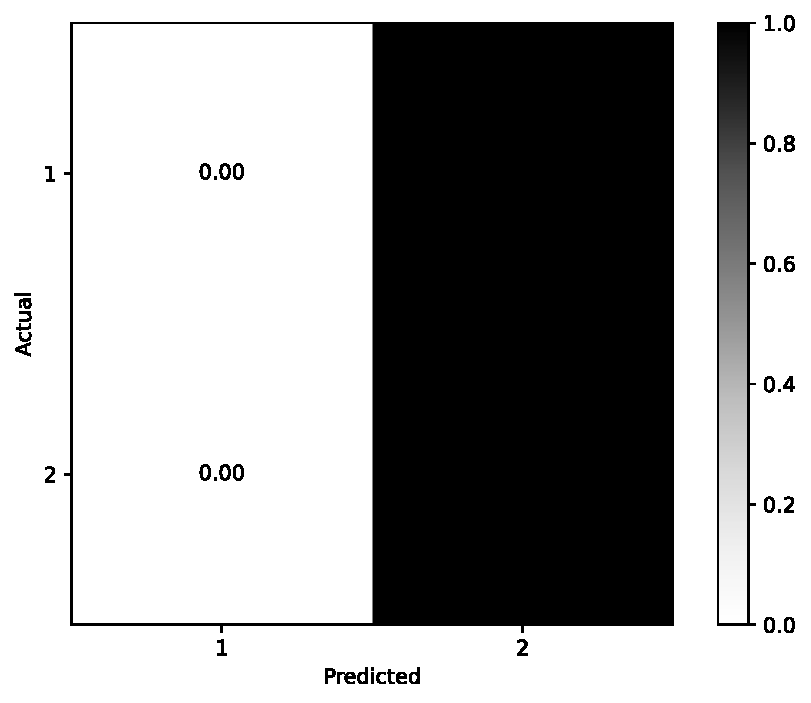
\includegraphics[width=\linewidth]{images/munich_num_classes_2_SimpleCNNSmall_confusion_matrix.pdf}
        \caption{SimpleCNNSmall - Confusion Matrix}
    \end{subfigure}

    \caption{Model comparison on the Munich binary task.}
\end{figure}

\section{Cross-Dataset Interpretation}

\begin{table}[H]
    \centering
    \begin{tabular}{|>{\raggedright\arraybackslash}p{3cm}|>{\raggedright\arraybackslash}p{2.6cm}|>{\raggedright\arraybackslash}p{7cm}|}
        \hline
        \textbf{Dataset} & \textbf{Best Current Model} & \textbf{Main Observation} \\
        \hline
        Aachen & FCNNNet / partially SimpleCNNSmall & Learnable structure exists, but one class is still poorly separated from the others. \\
        \hline
        MHH SeePain & None clearly robust & Binary task collapses to one class despite digital standardization. \\
        \hline
        MHH IDANA & FCNNNet & Highest discriminative capacity, but predictions remain concentrated on a narrow subset of labels; inconsistent data quality is a likely contributing factor. \\
        \hline
        Munich & None clearly robust & Binary task again collapses to one class, indicating insufficient robustness under low-data conditions. \\
        \hline
    \end{tabular}
    \caption{High-level interpretation of the reported experiments.}
    \label{tab:result_summary}
\end{table}

The overall picture is consistent across datasets. First, deeper fully connected models outperform the shallow baselines whenever any discriminative structure is learned at all. Second, class collapse remains the dominant failure mode for small tasks. Third, the present results should be interpreted as a strong baseline study rather than a final diagnostic system: they identify the bottlenecks of the current pipeline and clarify where the next research effort should be directed.

\chapter{Conclusion}

The current phase of the project successfully established an end-to-end experimental pipeline for pain drawing classification. The codebase now supports dataset conversion, tensor-based preprocessing, class balancing by undersampling, configurable experiment setup, model training, validation, confusion-matrix generation, and result visualization. This is an important milestone because it transforms heterogeneous clinical pain drawing data into a reproducible machine learning workflow.

From the experimental side, the results show that the task is meaningful but not yet solved. The Aachen and IDANA experiments demonstrate that neural networks can learn disease-related structure from pain drawings, particularly when the model has sufficient capacity. However, the confusion matrices also reveal that the learned decision boundaries are still unstable and that several diagnoses remain visually difficult to separate. In the IDANA setting, poor data-collection quality is also likely to be an important reason why stable patterns are difficult to learn. In the SeePain and Munich binary tasks, the current baselines collapse to a single-class solution, demonstrating that the present architectures are still not robust enough for these datasets.

Therefore, the main conclusion of this report is twofold. First, pain drawings clearly contain diagnostically relevant visual information, and the implemented pipeline is capable of extracting part of that structure. Second, the present architecture and training strategy are not yet adequate for robust clinical classification across all datasets. The next stage should therefore focus on stronger feature learning, better generalization, and improved handling of cross-dataset variability.

\chapter{Future Work}

\begin{itemize}
    \item Evaluate transfer learning with the already available ResNet-based models,
    \item Introduce data augmentation tailored to pain drawings while preserving clinical plausibility,
    \item Investigate cross-site generalization to measure robustness across Aachen, MHH, and Munich cohorts,
    \item Focus on obtaining higher-quality data, since better collection quality may be more beneficial than simply increasing dataset quantity,
    \item Expand the dataset and revisit currently excluded minority classes once sufficient sample sizes are available.
\end{itemize}

\begin{thebibliography}{9}

    \bibitem{litjens2017survey}
    G. Litjens et al., "A survey on deep learning in medical image analysis," \textit{Medical Image Analysis}, vol. 42, pp. 60--88, 2017.

    \bibitem{esteva2017dermatologist}
    A. Esteva et al., "Dermatologist-level classification of skin cancer with deep neural networks," \textit{Nature}, vol. 542, no. 7639, pp. 115--118, 2017.

    \bibitem{lecun2015deep}
    Y. LeCun, Y. Bengio, and G. Hinton, "Deep learning," \textit{Nature}, vol. 521, no. 7553, pp. 436--444, 2015.

    \bibitem{shen2017deep}
    D. Shen, G. Wu, and H.-I. Suk, "Deep learning in medical image analysis," \textit{Annual Review of Biomedical Engineering}, vol. 19, pp. 221--248, 2017.

    \bibitem{wester2020pain}
    L. Wester et al., "Pain drawings as a diagnostic tool...", 2020.

    \bibitem{emmert2018pain2d}
    D. Emmert et al., "A diagnostic support system...", 2018.

    \bibitem{rajgithub2026}
    R. Singh, "Analysis of Pain Drawings using Machine Learning," GitHub repository. Available: \url{https://github.com/rajasingh310/Analysis-of-Pain-Drawings-using-Machine-Learning}

\end{thebibliography}

\end{document}
